\documentclass{beamer}

\usepackage[T1]{fontenc}

\usepackage{graphicx}

\usepackage[normalem]{ulem}

\usepackage{newclude}

% Haskell
\usepackage[cache=false]{minted}

\usepackage{tikz}
\usetikzlibrary{shapes.geometric,positioning,shapes.symbols}

\usetheme{Madrid}

\title{Modular IDE}
\author{Nils Michael}
\date{\today}

\begin{document}

\frame{\titlepage}

\section{Plan}
\begin{frame}{Plan}
    \begin{itemize}
        \item Create an IDE
        \item Create Plugins
        \item ...
        \item Profit
    \end{itemize}
\end{frame}

\section{Create an IDE}
\begin{frame}{Create an IDE}
  So, here is my IDE:
\end{frame}

\begin{frame}{Example IDE}
\end{frame}

\begin{frame}{What does it have?}
  \begin{itemize}
    \item Loading of Plugins
    \item Unloading of Plugins?
    \item \sout{Optomizations}
  \end{itemize}
\end{frame}

\begin{frame}{Loading of Plugins}
  A Plugin, is a library, that is dynamically loaded,
  checked for a \textit{manifest}, which tells the IDE
  what functions this Plugin has.

  I have taken inspiration from Elm-Lang
\end{frame}

\begin{frame}{Plugin Architecture}
    \begin{figure}
        \centering
        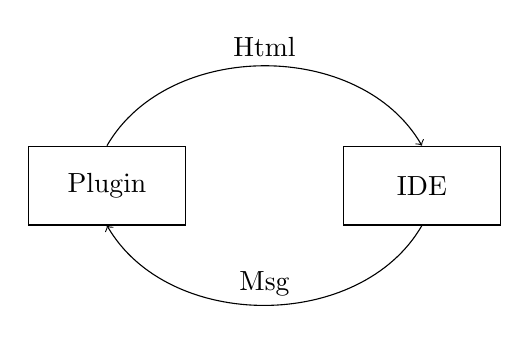
\begin{tikzpicture}
  % Nodes
  \node (p) [rectangle, draw, minimum height=1cm, minimum width=2cm] at (0, 0) {Plugin};
  \node (i) [rectangle, draw, minimum height=1cm, minimum width=2cm] at (4, 0) {IDE};
  % Arrow
  \draw[->] (p.north) to[out=60, in=120] node[midway, above] {Html} (i.north);
  \draw[->] (i.south) to[out=-120, in=-60] node[midway, above] {Msg} (p.south);
  % Header
\end{tikzpicture}


        \caption{Plugin Architecture}
    \end{figure}
\end{frame}

\begin{frame}{Plugin Example}
  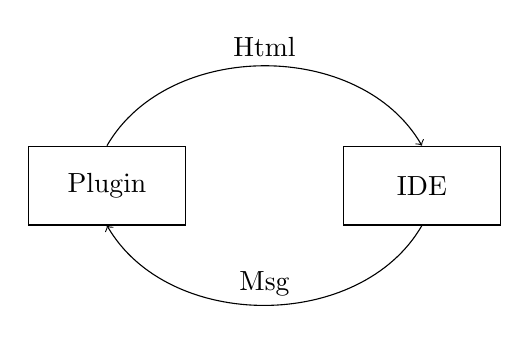
\begin{tikzpicture}
  % Nodes
  \node (p) [rectangle, draw, minimum height=1cm, minimum width=2cm] at (0, 0) {Plugin};
  \node (i) [rectangle, draw, minimum height=1cm, minimum width=2cm] at (4, 0) {IDE};
  % Arrow
  \draw[->] (p.north) to[out=60, in=120] node[midway, above] {Html} (i.north);
  \draw[->] (i.south) to[out=-120, in=-60] node[midway, above] {Msg} (p.south);
  % Header
\end{tikzpicture}


\end{frame}

\section{Remaining Work}
\begin{frame}{Plugins}
\begin{itemize}
  \item Make useful plugins
  \item Expand Plugin Language Landscape
\end{itemize}
\end{frame}

\begin{frame}{Remaining Work}
    \begin{figure}
        \centering
        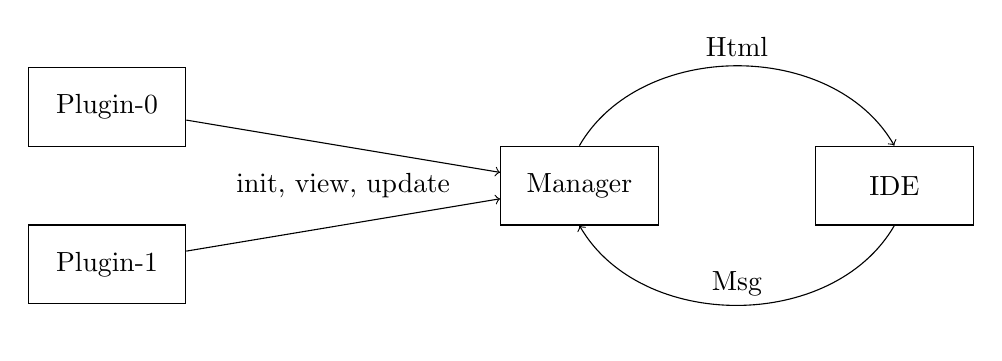
\begin{tikzpicture}
  % Nodes
  \node (p-0) [rectangle, draw, minimum height=1cm, minimum width=2cm] at (-5, 1) {Plugin-0};
  \node (p-1) [rectangle, draw, minimum height=1cm, minimum width=2cm] at (-5, -1) {Plugin-1};
  \node (m) [rectangle, draw, minimum height=1cm, minimum width=2cm] at (1, 0) {Manager};
  \node (i) [rectangle, draw, minimum height=1cm, minimum width=2cm] at (5, 0) {IDE};
  % Arrow
  \draw[->] (m.north) to[out=60, in=120] node[midway, above] {Html} (i.north);
  \draw[->] (i.south) to[out=-120, in=-60] node[midway, above] {Msg} (m.south);
  \draw[->] (p-0) -- (m) node[midway, above] {};
  \draw[->] (p-1) -- (m) node[midway, above] {};
  % Header
  \node (txt) at (-2, 0) {init, view, update};
\end{tikzpicture}


    \end{figure}
\end{frame}



\section{Remaining Work}
\begin{frame}{Tests}
\begin{itemize}
  \item Unit Tests
  \item Integration Tests
  \item Platform Tests
\end{itemize}
\end{frame}

\section{Remaining Work}
\begin{frame}{Cross Platform}
\begin{itemize}
  \item Figure out all necessary dependencies
  \item Ensure users can build for \textit{all} platforms
  \item Create installer?
\end{itemize}
\end{frame}

\section{Main Content}
\begin{frame}{Profit}
    \begin{figure}
        \centering
        \includegraphics[width=0.6\textwidth]{../../pics/grindset.png}
        \caption{Businessman}
    \end{figure}
\end{frame}
\end{document}
